\subsection{Ground Litter Decomposition Model}
Due to the irregular shape of ground litter, it is hard to represent ground litter as a special geometric. Therefore, we simplified it as the process of fungi decomposition of a plane, shown as follows.
\par
\begin{figure}[H]
  \label{figure2}
  \centering
  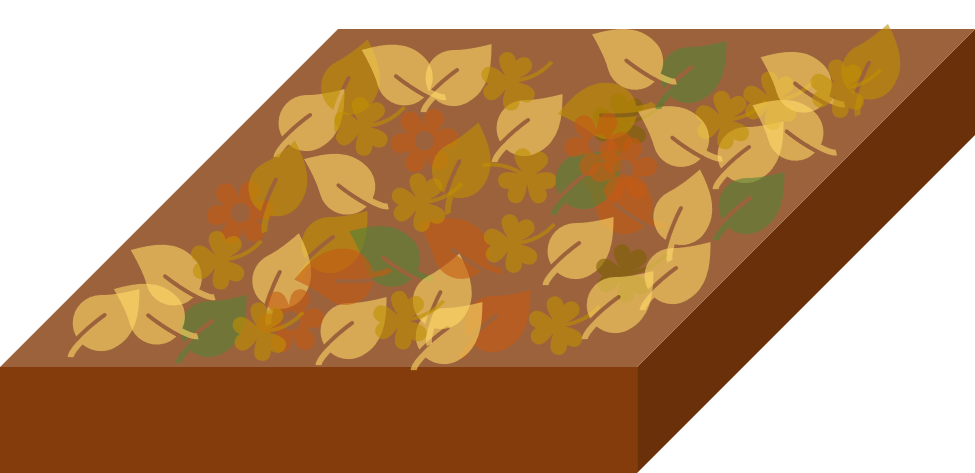
\includegraphics[width=0.55\textwidth]{figures/litter.png}
  \caption{Decomposition plane.}
\end{figure}
\par
Similar to the \textit{Woody Fibers Decomposition Model}, fungi that could decompose cellulose or lignin are distributed on a flat surface, gradually decomposing ground litter from outside to inside. By consulting the literature~\cite{literature}, the decomposition rate function of fungi decomposing ground litter on the plane is similar to the \textbf{logarithmic function} in \textit{Eq.~(\ref{eightheq})} as follows.
\begin{equation}
  \label{eightheq}
  DR \propto \ln (1+\frac{1}{4d})
\end{equation}
Combined with the analysis of environmental decomposition constant ($\varepsilon_{DR}$) and fungi activity factor ($ACT$) in \textit{Model~4.1}, we deduce the \textbf{decomposition rate of fungi in the plane distribution} as \textit{Eq.~(\ref{ninetheq})}
\begin{equation}
  \label{ninetheq}
  DR=\frac{\beta}{\varepsilon_{DR}} \ln (1+\frac{1}{4d}),\ d\in (0.05,\ +\infty)
\end{equation}
where $\beta$ represents fungi areal density, and $d$ represents the depth of fungi's current decomposition.
\par
Considering that fungal decomposing needs to be carried out at a certain distance below ground level, we set a lower limit of $0.05$ meters for the current depth of fungal decomposition, which avoids invalid information when $d\longrightarrow 0^+$, $DR\longrightarrow +\infty$.